%=========================================================
% Professional Black & White Beamer Template
% Compile using XeLaTeX
%=========================================================

\documentclass[aspectratio=169]{beamer}

%---------------------------------------------------------
% Theme
%---------------------------------------------------------
\usetheme{Madrid}
\usecolortheme{default}

%---------------------------------------------------------
% Font
%---------------------------------------------------------
\usepackage{fontspec}
\setmainfont{Times New Roman}
\setsansfont{Times New Roman}

%---------------------------------------------------------
% Packages
%---------------------------------------------------------
\usepackage{amsmath}
\usepackage{amssymb}
\usepackage{graphicx}
\usepackage{booktabs}
\usepackage{array}
\usepackage{multirow}
\usepackage[absolute,overlay]{textpos}

%---------------------------------------------------------
% Black & White Theme
%---------------------------------------------------------

\setbeamercolor{background canvas}{bg=white}

\setbeamercolor{normal text}{fg=black,bg=white}

\setbeamercolor{title}{fg=white,bg=black}
\setbeamercolor{frametitle}{fg=black,bg=white}

\setbeamercolor{author in head/foot}{fg=white,bg=black}
\setbeamercolor{title in head/foot}{fg=white,bg=black}
\setbeamercolor{date in head/foot}{fg=white,bg=black}

\setbeamercolor{block title}{fg=white,bg=black}
\setbeamercolor{block body}{fg=black,bg=white}

\setbeamercolor{item}{fg=black}
\setbeamercolor{enumerate item}{fg=black}
\setbeamercolor{section in toc}{fg=black}

\setbeamercolor{alerted text}{fg=black}

%---------------------------------------------------------
% Remove Navigation Icons
%---------------------------------------------------------

\setbeamertemplate{navigation symbols}{}

%---------------------------------------------------------
% Bullet Symbols
%---------------------------------------------------------

\setbeamertemplate{itemize item}{$\clubsuit$}
\setbeamertemplate{itemize subitem}{$\blacktriangleright$}
\setbeamertemplate{itemize subsubitem}{$\bullet$}
%\setbeamercovered{transparent}
\setbeamercovered{transparent=3} 
%---------------------------------------------------------
% Remove Header
%---------------------------------------------------------

\setbeamertemplate{headline}{}

%---------------------------------------------------------
% Footer
%---------------------------------------------------------

\setbeamertemplate{footline}
{
\leavevmode

\hbox{

\begin{beamercolorbox}[wd=.30\paperwidth,ht=2.8ex,dp=1ex,left]{author in head/foot}
\hspace{2mm}\insertshortauthor
\end{beamercolorbox}

\begin{beamercolorbox}[wd=.50\paperwidth,ht=2.8ex,dp=1ex,center]{title in head/foot}
\insertshorttitle
\end{beamercolorbox}

\begin{beamercolorbox}[wd=.20\paperwidth,ht=2.8ex,dp=1ex,right]{date in head/foot}
\insertframenumber/\inserttotalframenumber
\hspace{2mm}
\end{beamercolorbox}

}

}

%---------------------------------------------------------
% Logo Command
%---------------------------------------------------------

\newcommand{\MITELogo}{
\begin{textblock*}{2.3cm}(14.85cm,0.15cm)
    \includegraphics[width=1cm]{MITE_logo.png}
\end{textblock*}
}
\newcommand{\MITELogoTitle}{
\begin{textblock*}{8cm}(7.5cm,6cm)
    
\includegraphics[height=0.8cm]{images/MITE_logo.png}
\end{textblock*}
}
%---------------------------------------------------------
% Title Information
%---------------------------------------------------------

\title[\textbf{MLOps}]{\textbf{Machine Learning Operations}
}

\author[\textbf{Manjunath Prasad H. R.}]{\textbf{Manjunath Prasad H. R.} \\ Assistant Professor \\Department of Artificial Intelligence and Machine Learning}

\institute[\textbf{MITE}]{\textbf{Mangalore Institute of Technology and Engineering}}




\date{}
%=========================================================
\begin{document}
\MITELogoTitle
%=========================================================
% Title Slide (NO LOGO)
%=========================================================

\begin{frame}
\titlepage
\end{frame}

%=========================================================
% Table of Contents (NO LOGO)
%=========================================================

\begin{frame}{Outline}
\tableofcontents
\end{frame}

%=========================================================
\section{Course Description}



\begin{frame}{Course Description}
\begin{enumerate}%[<+->]
\item<1-> \textbf{Module 1:} Establish foundational understanding of MLOps practices, lifecycle management, and version control workflows using Git/GitHub for collaborative ML project tracking

\item<2-> \textbf{Module 2:} Execute systematic model development through data exploration, feature engineering, algorithm comparison, and implement reproducible experimentation tracking using MLflow

\item<3-> \textbf{Module 3:} Automate model training and testing through CI/CD pipelines (GitHub Actions), containerize models using Docker, and implement production deployment strategies

\item<4-> \textbf{Module 4:} Detect model degradation and drift in production, establish feedback loops for retraining, implement governance frameworks, and ensure regulatory compliance and responsible AI

\item<5-> \textbf{Module 5:} Apply end-to-end MLOps workflows to real-world scenarios including credit risk classification, recommendation engines with online learning, and continual learning pipelines
\end{enumerate}
\end{frame}

\section{Course Module Topics}
\subsection{Module Topics}
\begin{frame}{Course Module 1 Topics - Introduction to MLOps}
\begin{itemize}
\item  Defining MLOps and Its Challenges 
\item MLOps to Mitigate Risk 
\item MLOps for Scale 
\item People of MLOps 
\item Subject Matter Experts 
\item  Key MLOps Features 
\item  A Primer on Machine Learning 
\item  Model Development 
\item  Productionalization and Deployment
\item Monitoring 
\item   Iteration 
\item Life Cycle
Governance
\end{itemize}
\end{frame}

\subsection{Module Lab Component}
\begin{frame}{Module 1 Laboratory - Git Version Control}

\begin{itemize}

\item Set up GitHub/GitLab for ML project versioning.
\item Familiarize with Git commands.
\item Use Git for tracking model and code changes.

\end{itemize}

\end{frame}

\begin{frame}{Course Module 2 - Process in Model Development and Versioning}
\begin{itemize}

\item Machine Learning Model
\item ML Required Components
\item Different ML Algorithms
\item Different MLOps Challenges
\item Data Exploration
\item Feature Engineering and Selection
\item Experimentation
\item Evaluating and Comparing Models
\item Version Management
\item Reproducibility

\end{itemize}
\end{frame}

\begin{frame}{Module 2 Laboratory - Experiment Tracking with MLflow}

\begin{itemize}

\item Train a simple machine learning model (e.g., Logistic Regression).
\item Log model parameters using MLflow.
\item Log evaluation metrics.
\item Store model artifacts.
\item Compare different experiment runs.

\end{itemize}

\end{frame}

\begin{frame}{Course Module 3 - Preparing for Production and CI/CD Pipelining}
\begin{itemize}

\item Runtime Environments
\item Model Risk Evaluation
\item Quality Assurance for Machine Learning
\item Key Testing Considerations
\item Reproducibility and Auditability
\item Machine Learning Security
\item Model Risk Mitigation
\item Deploying to Production using CI/CD Pipelines
\item Building ML Artifacts
\item Deployment Strategies
\item Containerization
\item Scaling Deployments
\item Requirements and Challenges

\end{itemize}
\end{frame}


\begin{frame}{Module 3 Laboratory - CI/CD for ML Models}

\begin{itemize}
\item Set up a CI/CD pipeline using GitHub Actions.
\item Automate model training.
\item Automate model testing on code commits.
\item Validate reproducible ML workflows.
\end{itemize}

\end{frame}

\begin{frame}{Course Module 4 - Monitoring, Feedback Loop and Governance}
\begin{itemize}

\item Model Retraining
\item Understanding Model Degradation
\item Drift Detection in Practice
\item Feedback Loop
\item Model Governance
\item Matching Governance with Risk Level
\item Current Regulations
\item AI-Specific Regulations
\item Responsible Artificial Intelligence

\end{itemize}
\end{frame}

\begin{frame}{Module 4 Laboratory - Containerizing the Model}

\begin{itemize}

\item Train a simple ML model using Scikit-learn.
\item Save the trained model using Joblib or Pickle.
\item Develop a Flask or FastAPI application.
\item Serve the model as a REST API.
\item Create a Dockerfile.
\item Build the Docker image.
\item Run the Docker container.

\end{itemize}

\end{frame}

\begin{frame}{Course Module 5 - MLOps in Practice}
\begin{itemize}

\item Consumer Credit Risk Management
\item Model Development
\item Model Bias Consideration
\item Production Deployment
\item Marketing Recommendation Engines
\item Data Preparation
\item Experiment Management
\item Model Training
\item Model Deployment
\item Consumption Forecasting

\end{itemize}
\end{frame}

\begin{frame}{Module 5 Laboratory - Credit Risk Model}

\begin{itemize}

\item Use the German Credit Risk or Home Credit Default Risk dataset.
\item Train a classification model.
\item Apply Logistic Regression, Random Forest, or XGBoost.
\item Predict loan default probability.
\item Track the model lifecycle using MLflow.

\end{itemize}

\end{frame}


\begin{frame}{Module 5 Laboratory - Continual Learning Model}

\begin{itemize}

\item Train a recommendation engine using the MovieLens dataset.
\item Build an online learning pipeline.
\item Update the model using new user interactions.
\item Demonstrate continual learning in production.

\end{itemize}

\end{frame}

\section{Course Outcomes}
\begin{frame}{Course Outcomes}

\textbf{At the end of this course, the student will be able to:}

\vspace{0.4cm}

\begin{enumerate}

\item \textbf{UNDERSTAND} the fundamentals of MLOps, machine learning model deployment, and its significance.

\item \textbf{COMPARE} various model versioning techniques and experiment tracking methods.

\item \textbf{IMPLEMENT} model deployment strategies using Docker, Kubernetes, and cloud solutions.

\item \textbf{APPLY} machine learning models in production by detecting performance degradation and data/model drift.

\item \textbf{DEVELOP} an end-to-end MLOps workflow by integrating best practices in automation and testing.

\end{enumerate}

\end{frame}

\section{Textbook}
\begin{frame}{Textbook}
Mark Treveil et. al.  \textit{Introducing MLOps: 
How to Scale Machine Learning in the Enterprise}, O’Reilly 
Media, 2020
    \begin{figure}
        \centering
        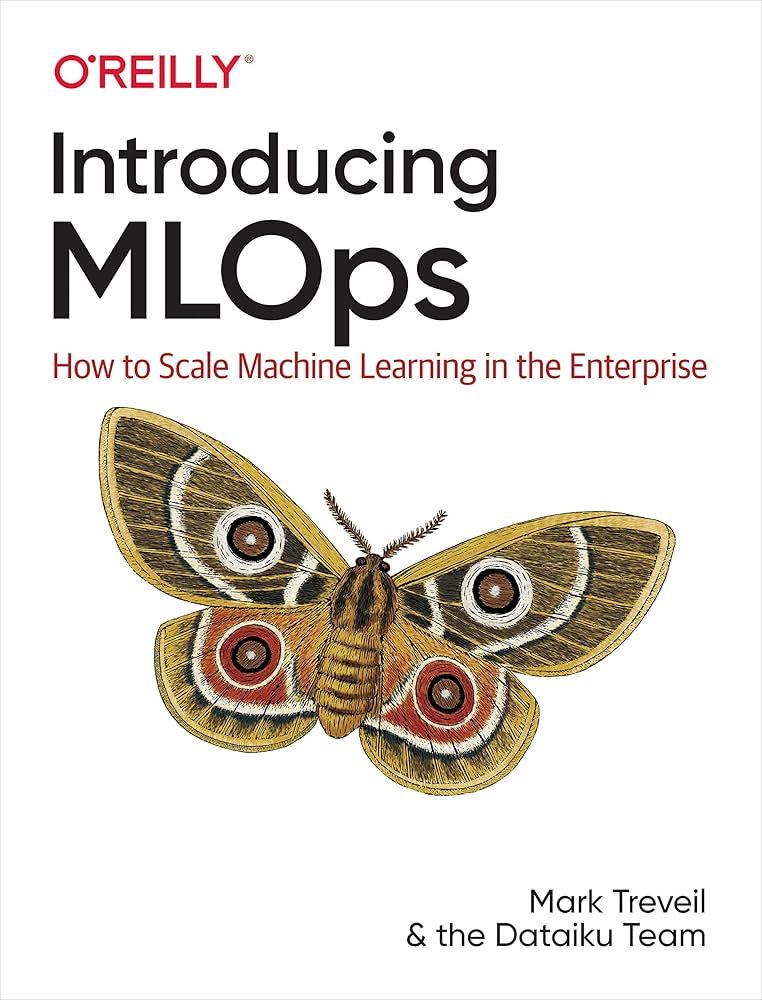
\includegraphics[width=0.30\linewidth]{images/Textbook.jpg}
        \caption{}
        \label{textbook}
    \end{figure}
\end{frame}

\subsection{Textbook Structure}
\begin{frame}{Textbook Structure}
Mark Treveil et. al.  \textit{Introducing MLOps: 
How to Scale Machine Learning in the Enterprise}, O’Reilly 
Media, 2020
    \begin{figure}
        \centering
        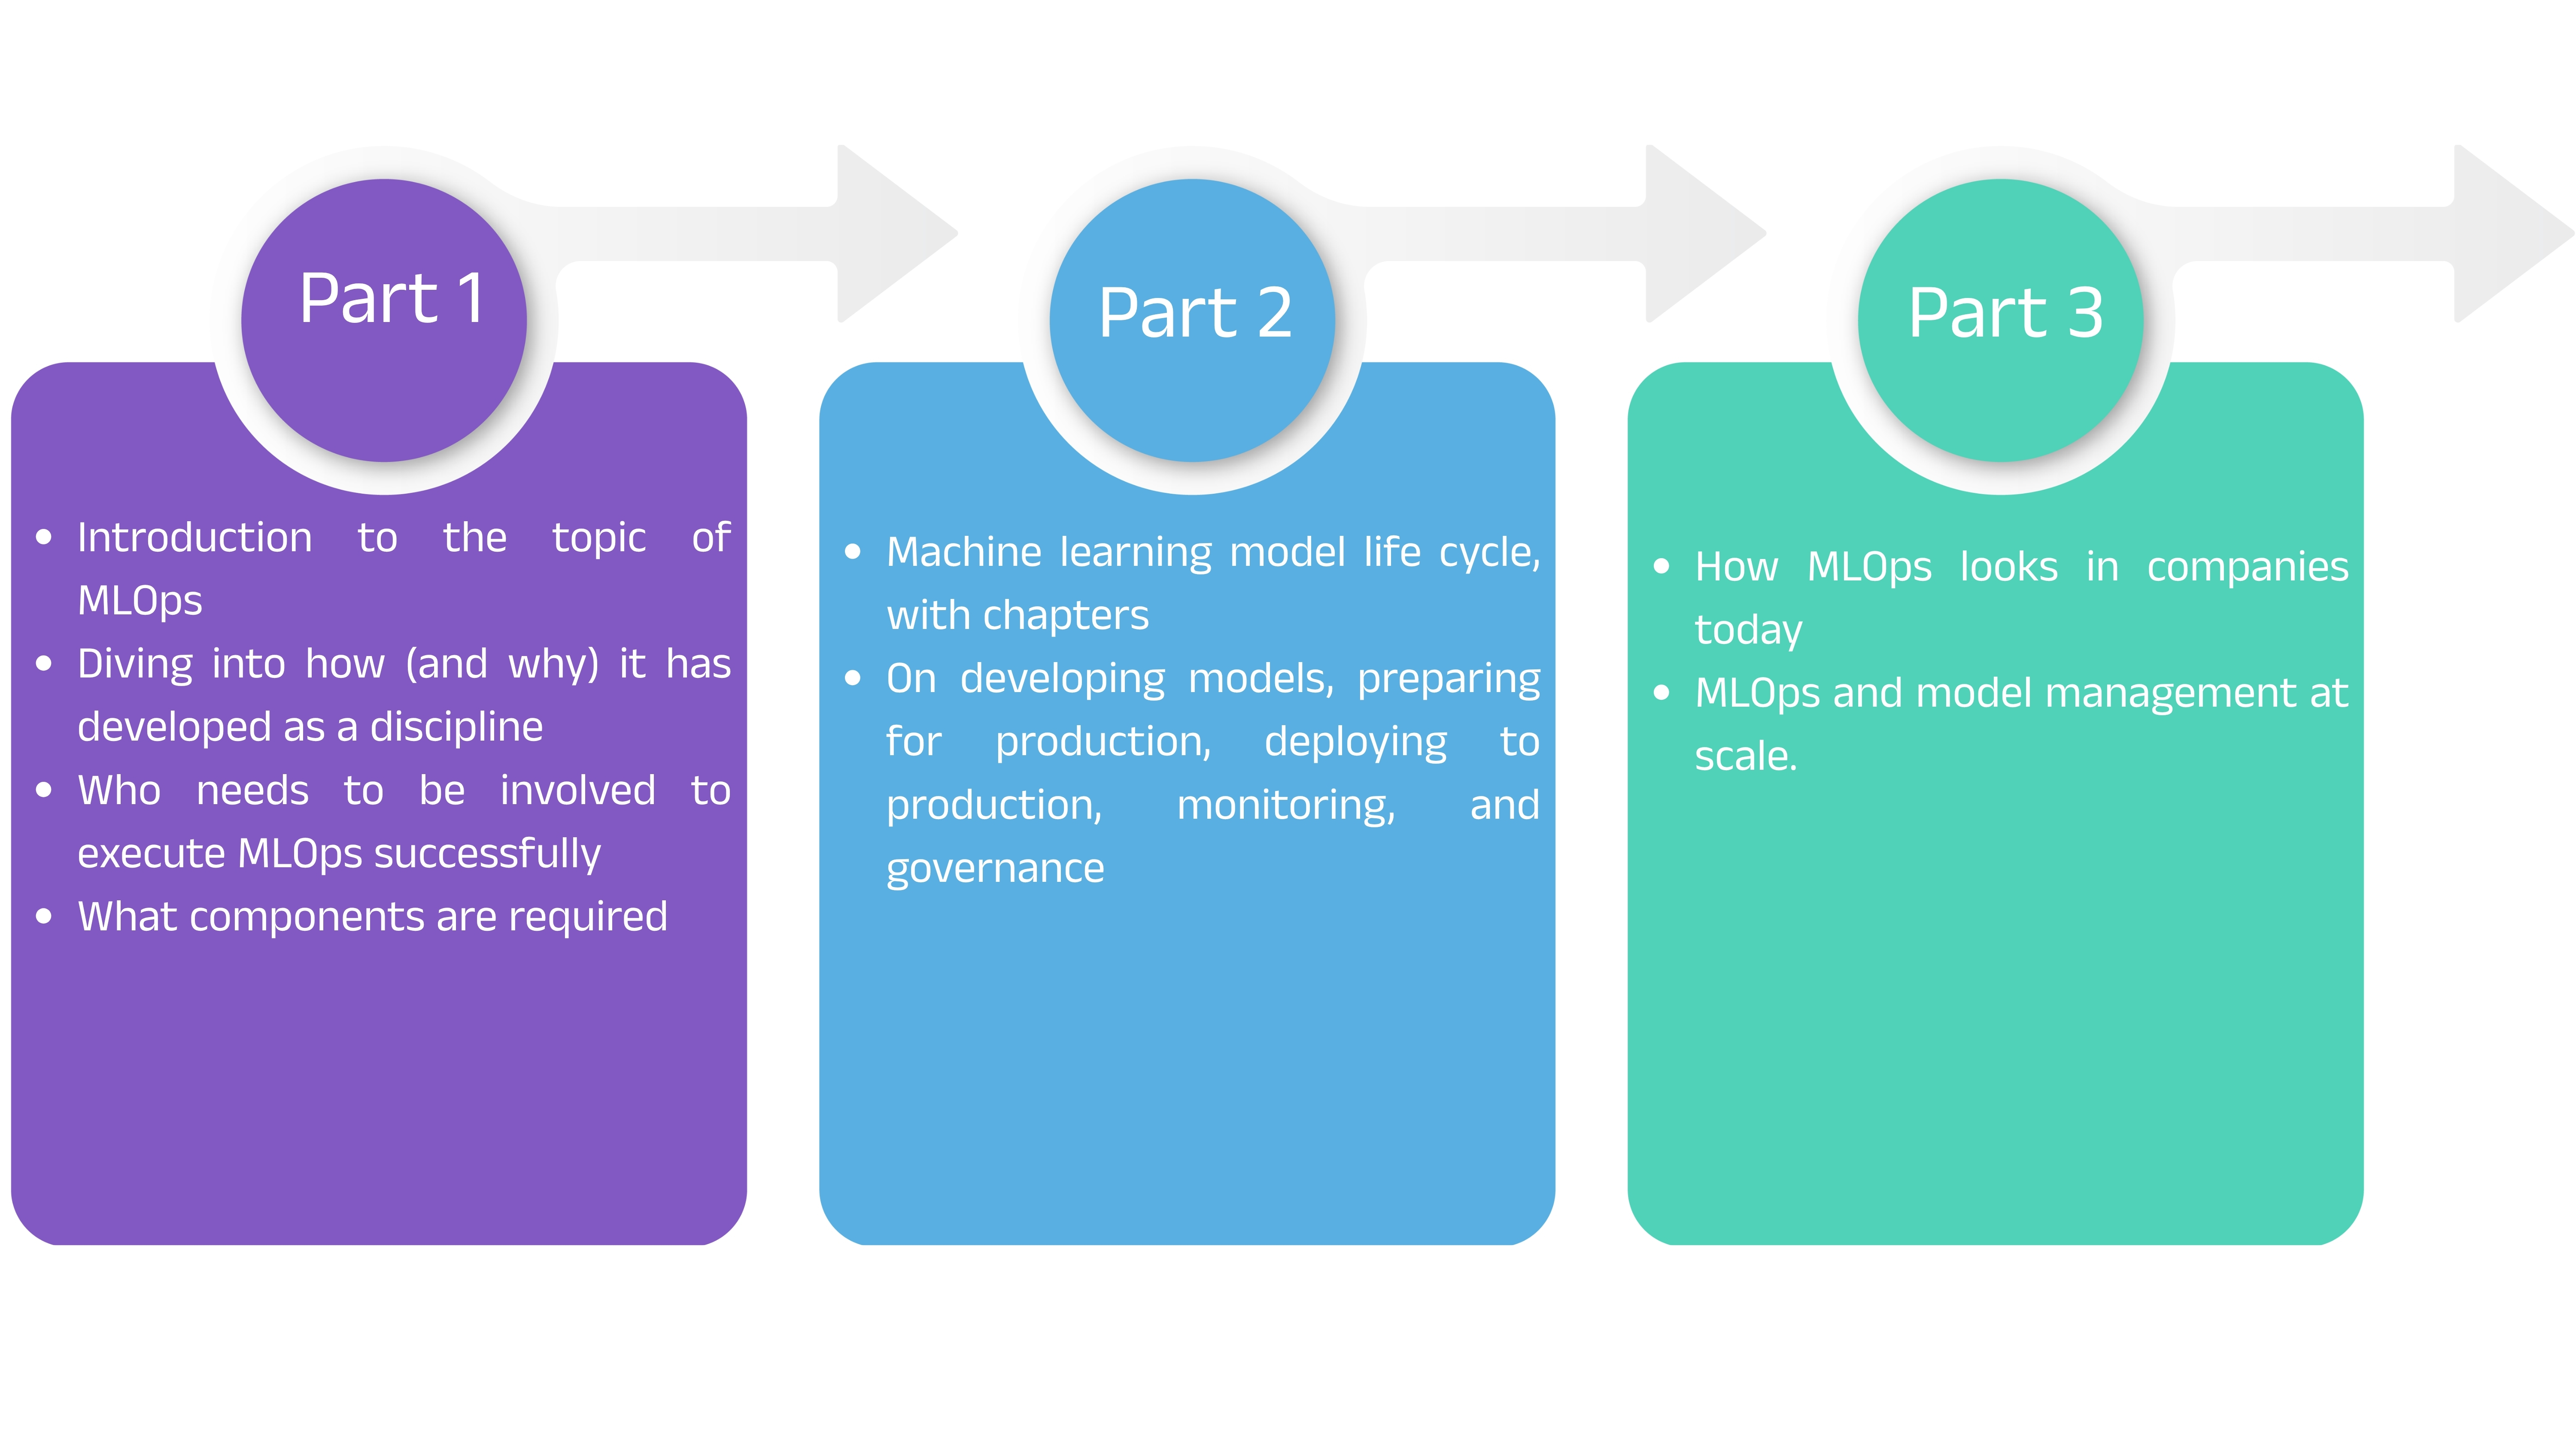
\includegraphics[scale=0.25]{images/Textbook_Structure.jpg}
    \end{figure}
\end{frame}
%---------------------------------------------------------
\begin{frame}{Technology Stack Used in this Course}

\small

\begin{table}[h]
\centering
\renewcommand{\arraystretch}{1.4}
\scriptsize
\begin{tabular}{|p{4cm}|p{3.5cm}|}
\hline
\textbf{Category} & \textbf{Tools} \\ \hline

Version Control & Git, GitHub \\ \hline

Programming & Python \\ \hline

ML Libraries & scikit-learn \\ \hline

Experiment Tracking & MLflow \\ \hline

API Development & FastAPI / Flask \\ \hline

Containers & Docker \\ \hline

CI/CD & GitHub Actions \\ \hline

Deployment & Docker Containers \\ \hline

Monitoring & MLflow, Custom Metrics \\ \hline

Data Handling & Pandas, NumPy \\ \hline

\end{tabular}
\end{table}
\vspace{0.4cm}

\textbf{Learning Outcome:}
\begin{itemize}
    \item Gain hands-on experience with an end-to-end MLOps toolchain.
    \item Learn how machine learning models are developed, deployed, monitored, and maintained in production.
\end{itemize}



\end{frame}

%=========================================================
% Thank You Slide
%=========================================================

\begin{frame}

% \MITELogo

\centering
\vfill

{\Huge Thank You}

\vfill

\end{frame}

%=========================================================

%=========================================================
% MODULE 1 : INTRODUCTION TO MLOps
% Textbook 1: Part I (Chapters 1, 2, 3)
% Mark Treveil et al., Introducing MLOps, O'Reilly, 2020
%=========================================================

%=========================================================
\section{Module 1: Why Now and Challenges}
%=========================================================

\begin{frame}{Introduction to MLOps}
\begin{block}{Machine Learning Operations (MLOps)}
A process that helps organizations and business leaders generate long-term value and reduce the risk associated with data science, machine learning, and AI initiatives.
\end{block}
\vspace{0.2cm}
\begin{enumerate}
\item<1-> MLOps is quickly becoming a \textbf{critical component} of successful data science project deployment in the enterprise.
\item<2-> It is a \textbf{relatively new concept}, yet it has seemingly skyrocketed into the data science lexicon overnight.
\item<3-> This chapter covers:
    \begin{itemize}
    \item What MLOps is at a high level and its challenges.
    \item Why it is essential to a successful data science strategy.
    \item Why it is coming to the forefront \textbf{now}.
    \end{itemize}
\end{enumerate}
\end{frame}

%---------------------------------------------------------
\begin{frame}{MLOps Versus ModelOps Versus AIOps}
\begin{enumerate}
\item<1-> \textbf{MLOps / ModelOps:} A new discipline that emerged under these names in late 2018 and 2019; the two terms are largely used \textbf{interchangeably}.
\item<2-> Some argue \textbf{ModelOps is more general} than MLOps, since it covers any kind of model (e.g., rule-based models), not only machine learning models.
\item<3-> This course focuses on the \textbf{machine learning model life cycle}, hence the term \textbf{``MLOps''}.
\item<4-> \textbf{AIOps} is an entirely different topic: solving operational challenges \textbf{using AI} (i.e., AI for DevOps).
\item<5-> \textbf{AIOps example:} Predictive maintenance for network failures, alerting DevOps teams to possible problems before they arise.
\end{enumerate}
\end{frame}

%---------------------------------------------------------
\begin{frame}{Growth of MLOps}
\begin{columns}[T]
\begin{column}{0.52\textwidth}
\begin{figure}
\centering
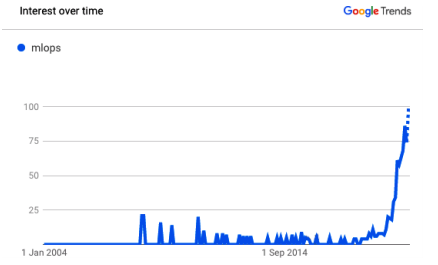
\includegraphics[width=\linewidth]{images/Fig1_1_mlops_growth.png}
\caption{Representation of the exponential growth of MLOps (not the parallel growth of the term ``ModelOps'')}
\end{figure}
\end{column}
\begin{column}{0.46\textwidth}
\begin{enumerate}\small
\item<1-> The chart shows Google Trends \textbf{interest over time} for the term ``mlops'' from 2004 onwards.
\item<2-> For more than a decade the interest remained \textbf{close to zero}, with only occasional spikes.
\item<3-> From around \textbf{2018--2019} the curve rises \textbf{exponentially}, reaching its peak (100).
\item<4-> This confirms MLOps as a \textbf{new and rapidly adopted} discipline in enterprise data science.
\end{enumerate}
\end{column}
\end{columns}
\end{frame}

%=========================================================
\subsection{Defining MLOps and Its Challenges}
%=========================================================

\begin{frame}{Defining MLOps}
\begin{block}{Definition}
At its core, MLOps is the \textbf{standardization and streamlining of machine learning life cycle management}.
\end{block}
\vspace{0.2cm}
\begin{enumerate}
\item<1-> From business problem to ML model, the steps at a very high level \textbf{seem straightforward}.
\item<2-> For most traditional organizations, developing \textbf{multiple ML models} and deploying them in production is \textbf{relatively new}.
\item<3-> Earlier, the number of models was manageable at a small scale, and there was less interest in understanding models and their dependencies company-wide.
\item<4-> With \textbf{decision automation} (decisions made without human intervention), models become more critical and \textbf{managing model risk} becomes a top-level concern.
\end{enumerate}
\end{frame}

%---------------------------------------------------------
\begin{frame}{Simple Machine Learning Model Life Cycle}
\begin{columns}[T]
\begin{column}{0.48\textwidth}
\begin{figure}
\centering
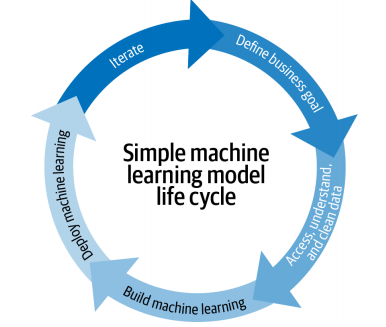
\includegraphics[width=\linewidth]{images/Fig1_2_simple_lifecycle.png}
\caption{A simple representation of the ML model life cycle, which often underplays the need for MLOps}
\end{figure}
\end{column}
\begin{column}{0.50\textwidth}
\begin{enumerate}\small
\item<1-> \textbf{Define business goal:} Identify the business problem the model must solve.
\item<2-> \textbf{Access, understand, and clean data:} Gather and prepare the data required.
\item<3-> \textbf{Build machine learning:} Train the ML model on the prepared data.
\item<4-> \textbf{Deploy machine learning:} Push the trained model into use.
\item<5-> \textbf{Iterate:} Repeat the cycle to improve the model.
\item<6-> This view \textbf{underplays} the real complexity of needs and tooling in an enterprise (see next figure).
\end{enumerate}
\end{column}
\end{columns}
\end{frame}

%---------------------------------------------------------
\begin{frame}{Challenges: Managing ML Life Cycles at Scale}
\begin{enumerate}
\item<1-> \textbf{There are many dependencies:}
    \begin{itemize}
    \item Data is constantly changing, and business needs shift as well.
    \item Results must be continually relayed back to the business to ensure the model in production meets the original goal.
    \end{itemize}
\item<2-> \textbf{Not everyone speaks the same language:}
    \begin{itemize}
    \item Business, data science, and IT teams are involved, but they do not use the same tools or share the same fundamental skills.
    \end{itemize}
\item<3-> \textbf{Data scientists are not software engineers:}
    \begin{itemize}
    \item They specialize in model building and assessment, not in writing applications.
    \item They juggle many roles; with staff turnover, they must manage models \textbf{they did not create}.
    \end{itemize}
\end{enumerate}
\end{frame}

%---------------------------------------------------------
\begin{frame}{Realistic Machine Learning Model Life Cycle}
\begin{columns}[T]
\begin{column}{0.42\textwidth}
\begin{figure}
\centering
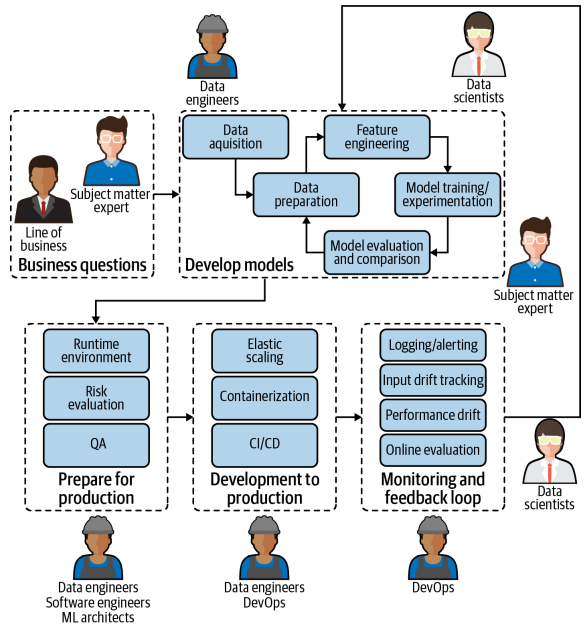
\includegraphics[height=0.64\textheight]{images/Fig1_3_realistic_lifecycle.png}
\caption{\scriptsize The realistic picture of an ML model life cycle inside an average organization today}
\end{figure}
\end{column}
\begin{column}{0.56\textwidth}
\begin{enumerate}\footnotesize
\item<1-> \textbf{Business questions:} Line of business and subject matter experts define the problem.
\item<2-> \textbf{Develop models:} Data acquisition $\rightarrow$ data preparation $\rightarrow$ feature engineering $\rightarrow$ model training/experimentation $\rightarrow$ model evaluation and comparison (data engineers, data scientists).
\item<3-> \textbf{Prepare for production:} Runtime environment, risk evaluation, QA (data engineers, software engineers, ML architects).
\item<4-> \textbf{Development to production:} Elastic scaling, containerization, CI/CD (data engineers, DevOps).
\item<5-> \textbf{Monitoring and feedback loop:} Logging/alerting, input drift tracking, performance drift, online evaluation (DevOps).
\item<6-> Feedback flows back to data scientists and SMEs; many people with \textbf{different skill sets and tools} are involved.
\end{enumerate}
\end{column}
\end{columns}
\end{frame}

%---------------------------------------------------------
\begin{frame}{MLOps and DevOps}
\begin{enumerate}
\item<1-> MLOps pulls heavily from \textbf{DevOps}, which streamlines the practice of software changes and updates.
\item<2-> Both center around:
    \begin{itemize}
    \item Robust automation and trust between teams.
    \item Collaboration and increased communication between teams.
    \item The end-to-end service life cycle (build, test, release).
    \item Prioritizing continuous delivery and high quality.
    \end{itemize}
\item<3-> \textbf{Critical difference:} Deploying software code is fundamentally different from deploying ML models.
\item<4-> Software code is \textbf{relatively static}, whereas data is \textbf{always changing}; models must constantly learn and adapt to new inputs.
\item<5-> ML models are made up of \textbf{both code and data}, which makes MLOps a new and unique discipline.
\end{enumerate}
\end{frame}

%---------------------------------------------------------
\begin{frame}{What About DataOps?}
\begin{enumerate}
\item<1-> \textbf{DataOps} was introduced in 2014 by IBM.
\item<2-> It seeks to provide \textbf{business-ready data} quickly, with focus on \textbf{data quality} and \textbf{metadata management}.
\item<3-> \textbf{Example:} If data a model relies on changes suddenly, DataOps alerts the business team and notifies the data team to investigate or revert a library upgrade and rebuild the partition.
\item<4-> MLOps \textbf{intersects} with DataOps, but goes further with additional key features (Chapter 3).
\item<5-> Until recently, teams could manage without centralized processes because they were not deploying ML models at scale.
\item<6-> Now, teams seek to formalize a \textbf{multi-stage, multi-discipline, multi-phase} process with a framework of MLOps best practices.
\end{enumerate}
\end{frame}

%=========================================================
\subsection{MLOps to Mitigate Risk}
%=========================================================

\begin{frame}{MLOps to Mitigate Risk}
\begin{enumerate}
\item<1-> MLOps is important to any team that has \textbf{even one model} in production.
\item<2-> Depending on the model, \textbf{continuous performance monitoring and adjusting} is essential.
\item<3-> By allowing safe and reliable operations, MLOps is key to \textbf{mitigating the risks} induced by ML models.
\item<4-> MLOps practices come at a \textbf{cost}; a proper \textbf{cost-benefit evaluation} should be performed for each use case.
\end{enumerate}
\end{frame}

%---------------------------------------------------------
\begin{frame}{Risk Assessment}
\begin{enumerate}
\item<1-> Risks vary widely: a monthly marketing recommendation engine is far lower stakes than a travel site whose \textbf{pricing and revenue} depend on an ML model.
\item<2-> A risk analysis should cover the risk that:
    \begin{itemize}
    \item The model is \textbf{unavailable} for a given period of time.
    \item The model returns a \textbf{bad prediction} for a given sample.
    \item Model \textbf{accuracy or fairness decreases} over time.
    \item The \textbf{skills} needed to maintain the model (data science talent) are lost.
    \end{itemize}
\item<3-> Risks are usually larger for models \textbf{deployed widely} and used outside the organization.
\item<4-> Risk assessment should be done at the \textbf{beginning} of each project and \textbf{reassessed periodically}.
\end{enumerate}
\end{frame}

%---------------------------------------------------------
\begin{frame}{Quantitative Risk Analysis: 5 $\times$ 5 Risk Matrix}
\begin{columns}[T]
\begin{column}{0.52\textwidth}
\begin{figure}
\centering
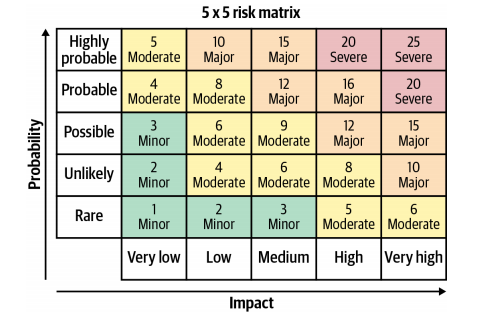
\includegraphics[width=\linewidth]{images/Fig1_4_risk_matrix.png}
\caption{A table that helps decision makers with quantitative risk analysis}
\end{figure}
\end{column}
\begin{column}{0.46\textwidth}
\begin{enumerate}\small
\item<1-> Risk is assessed on two metrics: \textbf{probability} (Rare $\rightarrow$ Highly probable) and \textbf{impact} (Very low $\rightarrow$ Very high).
\item<2-> Each is scored 1--5; their \textbf{product} gives the model's \textbf{severity} (1--25).
\item<3-> Severity is graded as \textbf{Minor}, \textbf{Moderate}, \textbf{Major}, or \textbf{Severe}.
\item<4-> Example: Possible (3) $\times$ High (4) = 12 $\rightarrow$ Major.
\item<5-> \textbf{Mitigation measures} are chosen based on this severity.
\end{enumerate}
\end{column}
\end{columns}
\end{frame}

%---------------------------------------------------------
\begin{frame}{Risk Mitigation}
\begin{enumerate}
\item<1-> MLOps becomes critical when a centralized team has \textbf{more than a handful} of operational models.
\item<2-> Without standardization, it is difficult to have a \textbf{global view} of the state of all models and take appropriate mitigation measures.
\item<3-> Full performance assessment is often only possible in the \textbf{production environment}.
\item<4-> Models are only as good as their training data; if production data changes, \textbf{performance may decrease rapidly}.
\item<5-> Model performance is sensitive to the \textbf{software environment} (versions of libraries such as scikit-learn, Python, or Linux) it runs in.
\item<6-> Deployment is \textbf{not the final step}; it is the beginning of monitoring the model and knowing how broadly it is used.
\end{enumerate}
\end{frame}

%---------------------------------------------------------
\begin{frame}{MLOps for Responsible AI}
\begin{enumerate}
\item<1-> \textbf{Intentionality:}
    \begin{itemize}
    \item Models are designed and behave in ways aligned with their purpose.
    \item Data comes from compliant and unbiased sources, with checks and balances on model bias.
    \item Includes \textbf{explainability}: results should be explainable by humans.
    \end{itemize}
\item<2-> \textbf{Accountability:}
    \begin{itemize}
    \item Centrally controlling, managing, and auditing the enterprise AI effort --- \textbf{no shadow IT}.
    \item Knowing which teams use what data, how, and in which models.
    \item Closely tied to \textbf{traceability}: where in the pipeline did something go wrong?
    \end{itemize}
\end{enumerate}
\end{frame}

%---------------------------------------------------------
\begin{frame}{Responsible AI and the Shift of Accountability}
\begin{enumerate}
\item<1-> ML models \textbf{lack the transparency} of traditional imperative code.
\item<2-> It is harder to understand which features determine a prediction, and to prove \textbf{regulatory compliance}.
\item<3-> Automation \textbf{shifts accountability} from the bottom of the hierarchy to the top.
\item<4-> Decisions once made by individuals (product price, loan approval) are now made by a model owned by a \textbf{data team manager or executive}.
\item<5-> Teams need good MLOps to practice Responsible AI, and Responsible AI \textbf{necessitates} MLOps strategies.
\end{enumerate}
\end{frame}

%=========================================================
\subsection{MLOps for Scale}
%=========================================================

\begin{frame}{MLOps for Scale}
\begin{enumerate}
\item<1-> MLOps is essential to \textbf{massively deploying} ML efforts and benefiting from economies of scale.
\item<2-> Going from a handful of models to \textbf{tens, hundreds, or thousands} requires MLOps discipline.
\item<3-> Good MLOps practices help teams, at a minimum, to:
    \begin{itemize}
    \item Keep track of \textbf{versioning}, especially with experiments in the design phase.
    \item Understand whether \textbf{retrained models are better} than previous versions, and promote better models to production.
    \item Ensure at defined periods (daily, monthly, etc.) that model performance is \textbf{not degrading} in production.
    \end{itemize}
\end{enumerate}
\end{frame}

%---------------------------------------------------------
\begin{frame}{Closing Thoughts}
\begin{enumerate}
\item<1-> MLOps practices are \textbf{not optional}; they are essential for scaling data science without putting the business at risk.
\item<2-> Without MLOps, teams face issues with \textbf{model quality and continuity}.
\item<3-> Worse, they may deploy models with real \textbf{negative business impact} (e.g., biased predictions).
\item<4-> Upper management should understand which models are in production and their business effect.
\item<5-> MLOps provides \textbf{transparency and accountability} down to the whole data pipeline (raw data to final output).
\end{enumerate}
\end{frame}

%=========================================================
\section{Module 1: People of MLOps}
%=========================================================

\begin{frame}{People of MLOps}
\begin{enumerate}
\item<1-> ML models are built primarily by data scientists, but MLOps involves \textbf{many roles} across the organization (see the realistic life cycle figure).
\item<2-> Each role has a different \textbf{skill set}, different \textbf{tools}, and a different \textbf{stake} in the model.
\item<3-> Key roles in MLOps:
    \begin{itemize}
    \item Subject Matter Experts (SMEs)
    \item Data Scientists and Data Engineers
    \item Software Engineers and DevOps
    \item Model Risk Manager / Auditor
    \item Machine Learning Architect
    \end{itemize}
\end{enumerate}
\end{frame}

%---------------------------------------------------------
\begin{frame}{Roles in MLOps and Their Responsibilities}
\small
\begin{table}
\centering
\renewcommand{\arraystretch}{1.25}
\scriptsize
\begin{tabular}{|p{3.2cm}|p{10cm}|}
\hline
\textbf{Role} & \textbf{Role in the ML Model Life Cycle} \\ \hline
Subject Matter Experts & Provide business questions, goals, and KPIs; evaluate whether model performance meets business needs. \\ \hline
Data Scientists & Build models that address the business question; deliver operationalizable models; assess model quality with SMEs. \\ \hline
Data Engineers & Optimize the retrieval and use of data to power ML models. \\ \hline
Software Engineers & Integrate ML models into the company's applications and systems. \\ \hline
DevOps & Build and test operational systems for security, performance, and availability; manage CI/CD pipelines. \\ \hline
Model Risk Manager/Auditor & Minimize overall risk from models in production; ensure compliance before deployment. \\ \hline
ML Architect & Ensure a scalable and flexible environment for ML pipelines from design to monitoring. \\ \hline
\end{tabular}
\end{table}
\end{frame}

%---------------------------------------------------------
\begin{frame}{Subject Matter Experts (SMEs)}
\begin{enumerate}
\item<1-> SMEs (line of business) \textbf{start the life cycle} by framing the business question.
\item<2-> They define \textbf{goals and KPIs} against which the model will ultimately be judged.
\item<3-> They bring \textbf{domain knowledge} needed during data exploration and feature engineering.
\item<4-> They evaluate whether model results are \textbf{useful for the business} and not just statistically good.
\item<5-> They take part in the \textbf{feedback loop}: monitoring results are relayed back to SMEs to confirm the model still meets the original goal.
\end{enumerate}
\end{frame}

%---------------------------------------------------------
\begin{frame}{Data Scientists and Data Engineers}
\begin{enumerate}
\item<1-> \textbf{Data Scientists:}
    \begin{itemize}
    \item Explore data, engineer features, train, evaluate, and compare models.
    \item Must deliver models that are \textbf{operationalizable}, reproducible, and explainable.
    \item Monitor model quality and drive retraining in the feedback loop.
    \end{itemize}
\item<2-> \textbf{Data Engineers:}
    \begin{itemize}
    \item Handle data acquisition and preparation pipelines.
    \item Ensure data is accessible, reliable, and available at the scale and speed required.
    \item Support preparing for production and deployment.
    \end{itemize}
\end{enumerate}
\end{frame}

%---------------------------------------------------------
\begin{frame}{Software Engineers and DevOps}
\begin{enumerate}
\item<1-> \textbf{Software Engineers:}
    \begin{itemize}
    \item Integrate ML models into applications and business systems.
    \item Ensure models work seamlessly with non-ML components.
    \end{itemize}
\item<2-> \textbf{DevOps:}
    \begin{itemize}
    \item Build and operate production systems: runtime, containerization, elastic scaling.
    \item Own \textbf{CI/CD pipelines} for automated testing and deployment.
    \item Monitor resource usage, latency, logging, and alerting in production.
    \end{itemize}
\end{enumerate}
\end{frame}

%---------------------------------------------------------
\begin{frame}{Model Risk Manager/Auditor and ML Architect}
\begin{enumerate}
\item<1-> \textbf{Model Risk Manager / Auditor:}
    \begin{itemize}
    \item Minimizes the overall risk to the company from models in production.
    \item Ensures compliance with internal and external (regulatory) requirements.
    \item Reviews documentation, validation, and sign-offs before deployment.
    \end{itemize}
\item<2-> \textbf{Machine Learning Architect:}
    \begin{itemize}
    \item Designs a scalable and flexible environment for ML pipelines.
    \item Selects and introduces technologies that improve performance in production.
    \item Bridges data science, data engineering, and IT infrastructure.
    \end{itemize}
\end{enumerate}
\end{frame}

%=========================================================
\section{Module 1: Key MLOps Features}
%=========================================================

\begin{frame}{Key MLOps Features}
\begin{enumerate}
\item<1-> MLOps affects many roles and many parts of the ML life cycle.
\item<2-> The \textbf{five key components} of MLOps are:
    \begin{enumerate}
    \item Development
    \item Deployment
    \item Monitoring
    \item Iteration
    \item Governance
    \end{enumerate}
\item<3-> These are introduced here at a high level and form the foundation for Chapters 4--8.
\end{enumerate}
\end{frame}

%=========================================================
\subsection{A Primer on Machine Learning}
%=========================================================

\begin{frame}{A Primer on Machine Learning}
\begin{block}{Machine Learning}
The science of computer algorithms that automatically \textbf{learn and improve from experience} rather than being explicitly programmed.
\end{block}
\vspace{0.1cm}
\begin{enumerate}
\item<1-> Algorithm selection has a \textbf{direct impact} on MLOps processes.
\item<2-> Algorithms analyze sample data (\textbf{training data}) to build a model that makes predictions.
\item<3-> \textbf{Examples:} Identifying an electricity meter type from a photo; recommending insurance products based on behavior of similar customers.
\item<4-> On \textbf{unseen data}, the model predicts assuming it is related to the previous data.
\item<5-> Models range from simple \textbf{decision trees} and \textbf{logistic regression} to complex \textbf{deep learning} models.
\end{enumerate}
\end{frame}

%=========================================================
\subsection{Model Development}
%=========================================================

\begin{frame}{Model Development: Establishing Business Objectives}
\begin{enumerate}
\item<1-> Development starts with a \textbf{business objective}, e.g., reducing fraudulent transactions to $<$ 0.1\% or identifying faces in social media photos.
\item<2-> Objectives come with performance targets, infrastructure requirements, and cost constraints, captured as \textbf{KPIs}.
\item<3-> KPIs enable the business performance of models in production to be \textbf{monitored}.
\item<4-> ML projects are part of a larger project that impacts technologies, processes, and people, so objectives include \textbf{change management}.
\item<5-> The required degree of \textbf{transparency} strongly influences the choice of algorithm and the need to explain predictions.
\end{enumerate}
\end{frame}

%---------------------------------------------------------
\begin{frame}{Data Sources and Exploratory Data Analysis}
\small
\begin{enumerate}
\item<1-> SMEs and data scientists begin by searching for suitable input data --- often the \textbf{most arduous} part of the journey.
\item<2-> \textbf{Key questions for finding data:}
    \begin{itemize}
    \item What relevant datasets are available? Are they accurate and reliable?
    \item How can stakeholders access the data? What \textbf{features} can be made by combining sources?
    \item Will the data be available in real time?
    \item Is labeling with ``ground truth'' needed, or does unsupervised learning make sense? At what cost?
    \end{itemize}
\item<3-> \textbf{More questions:}
    \begin{itemize}
    \item What platform should be used? How will data be updated after deployment?
    \item Will the model's use reduce the \textbf{representativeness} of the data?
    \item How will the KPIs be measured?
    \end{itemize}
\end{enumerate}
\end{frame}

%---------------------------------------------------------
\begin{frame}{Data Governance Questions and EDA}
\begin{enumerate}
\item<1-> \textbf{Data governance constraints} raise more questions:
    \begin{itemize}
    \item Can the datasets be used for this purpose? What are the terms of use?
    \item Is there \textbf{PII} that must be redacted or anonymized?
    \item Are there features (e.g., gender) that legally cannot be used?
    \item Are minority populations represented well enough for equivalent performance?
    \end{itemize}
\item<2-> \textbf{Exploratory Data Analysis (EDA)} helps to:
    \begin{itemize}
    \item Build hypotheses about the data.
    \item Identify data cleaning requirements.
    \item Inform the selection of potentially significant features.
    \end{itemize}
\item<3-> EDA can be done \textbf{visually} for intuition or \textbf{statistically} for rigor.
\end{enumerate}
\end{frame}

%---------------------------------------------------------
\begin{frame}{Feature Engineering and Selection; Training and Evaluation}
\begin{enumerate}
\item<1-> \textbf{Feature engineering} transforms raw data into ``features'' that better represent the underlying problem.
\item<2-> Features are \textbf{arrays of numbers of fixed size} --- the only object ML algorithms understand.
\item<3-> It includes \textbf{data cleansing}, often the largest part of an ML project in time spent.
\item<4-> \textbf{Training} is iterative: test algorithms, generate features, adapt selections, tune hyperparameters; it is the most \textbf{compute-intensive} step.
\item<5-> An \textbf{experiment tracking tool} records data, features, parameters, and metrics so experiments can be compared side-by-side.
\item<6-> The best solution needs \textbf{quantitative} (accuracy, error) and \textbf{qualitative} (explainability, ease of deployment) criteria.
\end{enumerate}
\end{frame}

%---------------------------------------------------------
\begin{frame}{Reproducibility}
\begin{enumerate}
\item<1-> Many experiments are short-lived, but \textbf{significant versions} of a model must be saved.
\item<2-> \textbf{Reproducibility} aims to save enough about the environment so the model can be \textbf{reproduced with the same results from scratch}.
\item<3-> Without it, data scientists cannot confidently iterate on models.
\item<4-> Nor can they hand the model to \textbf{DevOps} to check that the lab result is faithfully reproduced in production.
\item<5-> True reproducibility requires \textbf{version control of all assets and parameters}, including training/evaluation data and the software environment.
\end{enumerate}
\end{frame}

%---------------------------------------------------------
\begin{frame}{Responsible AI in Model Development}
\begin{enumerate}
\item<1-> DevOps must understand how to \textbf{verify} the model: what it does, how to test it, expected results.
\item<2-> Regulated industries must document how the model was built and tuned; critical models may be \textbf{independently rebuilt}.
\item<3-> \textbf{Documentation} is the standard solution; automated model documentation helps, but some must be written by hand.
\item<4-> Standard performance measures do not explain \textbf{how} predictions are made.
\item<5-> The ``how'' is needed to sanity-check the model, improve features, and ensure \textbf{fairness} (sex, age, race) --- the field of \textbf{explainability}.
\end{enumerate}
\end{frame}

%---------------------------------------------------------
\begin{frame}{Explainability Techniques}
\begin{enumerate}
\item<1-> \textbf{Partial dependence plots:} Look at the marginal impact of features on the predicted outcome.
\item<2-> \textbf{Subpopulation analyses:} Look at how the model treats specific subpopulations; the basis of many fairness analyses.
\item<3-> \textbf{Individual model predictions (e.g., Shapley values):} Explain how each feature value contributes to a specific prediction.
\item<4-> \textbf{What-if analysis:} Helps the user understand the sensitivity of the prediction to its inputs.
\item<5-> MLOps work done up front in development makes models \textbf{easier to manage} later, especially in production.
\end{enumerate}
\end{frame}

%=========================================================
\subsection{Productionalization and Deployment}
%=========================================================

\begin{frame}{Productionalization and Deployment}
\begin{enumerate}
\item<1-> Presents an \textbf{entirely different} set of technical challenges than model development.
\item<2-> It is the domain of the \textbf{software engineer} and the \textbf{DevOps team}.
\item<3-> Information exchange between data scientists and these teams must not be underestimated.
\item<4-> Without effective collaboration, \textbf{delays or failures to deploy} are inevitable.
\end{enumerate}
\end{frame}

%---------------------------------------------------------
\begin{frame}{Model Deployment Types and Contents}
\begin{enumerate}
\item<1-> \textbf{Model-as-a-service (live-scoring model):} Deployed in a framework providing a \textbf{REST API endpoint} that responds to requests in real time.
\item<2-> \textbf{Embedded model:} Packaged into an application which is then published, e.g., an application providing \textbf{batch-scoring}.
\item<3-> A deployed model comprises \textbf{code} (Python, R, or Java) and \textbf{data artifacts}, with version dependencies on runtimes and packages.
\item<4-> Different versions in production \textbf{may cause predictions to differ}.
\item<5-> \textbf{Portable formats} (PMML, PFA, ONNX, POJO) reduce dependencies, but support limited algorithms and may behave subtly differently.
\end{enumerate}
\end{frame}

%---------------------------------------------------------
\begin{frame}{Containerization}
\begin{enumerate}
\item<1-> An increasingly popular solution to \textbf{dependency headaches} when deploying ML models.
\item<2-> Container technologies such as \textbf{Docker} are lightweight alternatives to virtual machines.
\item<3-> Applications run in \textbf{independent, self-contained environments} matching each model's exact requirements.
\item<4-> Enable new models to be seamlessly deployed using the \textbf{blue-green deployment} technique.
\item<5-> Compute can be \textbf{scaled elastically} using multiple containers.
\item<6-> Orchestration of many containers is handled by \textbf{Kubernetes}, in the cloud or on-premise.
\end{enumerate}
\end{frame}

%---------------------------------------------------------
\begin{frame}{Model Deployment Requirements}
\begin{enumerate}
\item<1-> \textbf{Rapid, automated deployment} is always preferred to labor-intensive processes.
\item<2-> For \textbf{short-lifetime, self-service} applications, a fully automated single-step push-to-production may be adequate (resources capped by Linux cgroups; simple UIs with Flask).
\item<3-> For \textbf{customer-facing, mission-critical} use cases, a robust \textbf{CI/CD pipeline} is required.
\item<4-> In heavily regulated industries (finance, pharmaceuticals), checks are extensive and may involve \textbf{manual intervention}.
\item<5-> MLOps, like DevOps, aims to \textbf{automate CI/CD} as far as possible: faster deployment, more regression testing, fewer errors.
\end{enumerate}
\end{frame}

%---------------------------------------------------------
\begin{frame}{Robust CI/CD Pipeline for Mission-Critical Models}
\begin{enumerate}
\item<1-> Ensuring all coding, documentation, and sign-off standards have been met.
\item<2-> Re-creating the model in something approaching the production environment.
\item<3-> Revalidating the model accuracy.
\item<4-> Performing explainability checks.
\item<5-> Ensuring all governance requirements have been met.
\item<6-> Checking the quality of any data artifacts.
\item<7-> Testing resource usage under load.
\item<8-> Embedding into a more complex application, including integration tests.
\end{enumerate}
\end{frame}

%=========================================================
\subsection{Monitoring}
%=========================================================

\begin{frame}{Monitoring}
\begin{enumerate}
\item<1-> After deployment, the model must \textbf{continue to perform well} over time.
\item<2-> Good performance means different things to \textbf{DevOps}, \textbf{data scientists}, and the \textbf{business}.
\item<3-> \textbf{DevOps concerns:}
    \begin{itemize}
    \item Is the model getting the job done \textbf{quickly enough}?
    \item Is it using a sensible amount of \textbf{memory and processing time}?
    \end{itemize}
\item<4-> This is traditional IT performance monitoring; ML resource demands are similar to traditional software.
\item<5-> Scalability matters, e.g., when \textbf{retraining in production}; deep learning needs more resources than decision trees.
\end{enumerate}
\end{frame}

%---------------------------------------------------------
\begin{frame}{Data Scientist Concerns}
\begin{enumerate}
\item<1-> ML models \textbf{degrade over time}, since they are models of the data they were trained on --- a problem not faced by traditional software.
\item<2-> The real world does not stand still:
    \begin{itemize}
    \item A fraud model trained six months ago will not reflect a \textbf{new type of fraud}.
    \item An ad model becomes less relevant if a website attracts a \textbf{younger user base}.
    \end{itemize}
\item<3-> When performance becomes unacceptable, \textbf{retraining} is necessary.
\item<4-> Retraining frequency depends on how fast the world changes, accuracy needed, and ease of building/deploying a better model.
\item<5-> Two approaches to detect degradation: \textbf{ground truth} and \textbf{input drift}.
\end{enumerate}
\end{frame}

%---------------------------------------------------------
\begin{frame}{Ground Truth and Input Drift}
\begin{enumerate}
\item<1-> \textbf{Ground truth:} The correct answer to the question the model was asked (e.g., ``Is this transaction actually fraudulent?'').
\item<2-> Sometimes obtained \textbf{rapidly} (ad clicks within seconds); often \textbf{slowly} (fraud reported up to a month later, or never).
\item<3-> Slow ground truth prevents accurate daily monitoring; if rapid feedback is needed, use input drift.
\item<4-> \textbf{Input drift:} If recent requests differ distinctly from training data, model performance is likely compromised.
\item<5-> All required data \textbf{already exists} --- no need to wait for ground truth.
\item<6-> Drift identification brings \textbf{agility} to enterprise AI efforts (detailed in Chapter 7).
\end{enumerate}
\end{frame}

%---------------------------------------------------------
\begin{frame}{Business Concerns}
\begin{enumerate}
\item<1-> The business takes a \textbf{holistic} view:
    \begin{itemize}
    \item Is the model delivering \textbf{value} to the enterprise?
    \item Do benefits outweigh the \textbf{cost} of developing and deploying it?
    \end{itemize}
\item<2-> The original \textbf{KPIs} should be monitored, automatically where possible --- rarely trivial.
\item<3-> Even monitoring fraud rate does not answer: what is the \textbf{net gain in dollars}?
\item<4-> In the absence of a ``dollar-o-meter,'' monitoring \textbf{business KPIs} is the best option.
\item<5-> Choose a \textbf{baseline} that isolates ML value, e.g., compare against a \textbf{rule-based} model built from subject matter expertise.
\end{enumerate}
\end{frame}

%=========================================================
\subsection{Iteration and Life Cycle}
%=========================================================

\begin{frame}{Iteration and Life Cycle}
\begin{enumerate}
\item<1-> Developing and deploying \textbf{improved versions} is essential and one of the more challenging parts of MLOps.
\item<2-> Reasons for a new version: \textbf{model drift}, refined business objectives/KPIs, or a \textbf{better model design}.
\item<3-> In fast-moving environments, daily retraining and redeployment are often \textbf{automated}.
\item<4-> Pitfalls even in simple retraining:
    \begin{itemize}
    \item Does the new training data look as expected? (automated validation)
    \item Is the data complete and consistent?
    \item Are feature distributions similar to the previous training set?
    \end{itemize}
\item<5-> Compare new and live model metrics on the \textbf{same dataset}; if variation is wide, seek \textbf{manual intervention}.
\end{enumerate}
\end{frame}

%---------------------------------------------------------
\begin{frame}{Retraining Scenarios}
\begin{enumerate}
\item<1-> Even ``simple'' retraining needs multiple datasets: scoring data reconciliation (with ground truth), cleaning/validation, the previous model, and checks.
\item<2-> Other scenarios are more complicated, making \textbf{automated redeployment unlikely}.
\item<3-> \textbf{Drift-motivated retraining:} If new labeled data exists, retraining with it has the best cost-benefit ratio.
\item<4-> If ground truth is slow, there may be \textbf{little new labeled data}.
\item<5-> Data scientists must understand the drift, \textbf{adjust existing training data}, and design mitigations (e.g., remove a feature, resample rows).
\item<6-> Time needed grows with the amount of \textbf{modeling debt}.
\end{enumerate}
\end{frame}

%---------------------------------------------------------
\begin{frame}{The Feedback Loop: Shadow Testing and A/B Testing}
\begin{enumerate}
\item<1-> The live scoring and retraining environments are usually \textbf{distinct}, so evaluation in retraining may be compromised.
\item<2-> \textbf{Shadow testing:} New version runs alongside the incumbent; the incumbent answers, the new version's results are only \textbf{logged}, then compared statistically.
\item<3-> Shadow scoring gives SMEs visibility on future versions for a \textbf{smoother transition}.
\item<4-> When outcomes depend on the user's reaction (ad clicks), \textbf{A/B testing} is more common.
\item<5-> \textbf{A/B testing:} Requests are \textbf{split} between the two models; each request is processed by only one model.
\end{enumerate}
\end{frame}

%---------------------------------------------------------
\begin{frame}{A/B Testing Variants}
\begin{enumerate}
\item<1-> Statistically meaningful A/B conclusions require \textbf{careful planning}.
\item<2-> \textbf{Fixed-horizon test:} Wait until a predetermined number of samples is tested; ``peeking'' early is \textbf{unreliable}.
\item<3-> In a live commercial environment, every bad prediction costs money, so not stopping early can be \textbf{expensive}.
\item<4-> \textbf{Bayesian / multi-armed bandit tests} aim to draw conclusions \textbf{more quickly}.
\item<5-> Multi-armed bandit testing is \textbf{adaptive}: traffic to underperforming models is reduced, lowering business cost.
\end{enumerate}
\end{frame}

%---------------------------------------------------------
\begin{frame}{Iterating on the Edge}
\begin{enumerate}
\item<1-> Iterating on models deployed to \textbf{millions of devices} (phones, sensors, cars) poses different challenges.
\item<2-> \textbf{Centralized training:} Relay feedback to a central point. Tesla's autopilot (500,000+ cars) retrains about 50 neural networks using 70,000 GPU hours.
\item<3-> \textbf{Federated learning:} Google's GBoard retrains locally on each phone and sends a summary of improvements, which are averaged into the shared model.
\item<4-> Benefits of federated learning:
    \begin{itemize}
    \item Personal data need not be collected centrally.
    \item Improved model is usable immediately on each phone.
    \item Overall power consumption goes down.
    \end{itemize}
\end{enumerate}
\end{frame}

%=========================================================
\subsection{Governance}
%=========================================================

\begin{frame}{Governance}
\begin{block}{Governance}
The set of controls placed on a business to ensure that it delivers on its responsibilities to all stakeholders --- shareholders, employees, the public, and national governments.
\end{block}
\vspace{0.1cm}
\begin{enumerate}
\item<1-> Responsibilities include \textbf{financial, legal, and ethical} obligations, all underpinned by \textbf{fairness}.
\item<2-> \textbf{Legal obligations} existed before ML: financial regulations protect against fraud; pharmaceutical rules safeguard public health.
\item<3-> Broader legislation protects vulnerable sectors and ensures a level playing field on sex, race, age, or religion.
\item<4-> Data regulations such as \textbf{GDPR (2016, EU)} and \textbf{CCPA (2018, California)} have had immense impact on ML.
\end{enumerate}
\end{frame}

%---------------------------------------------------------
\begin{frame}{GDPR Principles}
\begin{enumerate}
\item<1-> GDPR sets principles for \textbf{processing personal data} (collection, storage, alteration, use); CCPA closely mirrors them.
\item<2-> The principles are:
    \begin{itemize}
    \item Lawfulness, fairness, and transparency
    \item Purpose limitation
    \item Data minimization
    \item Accuracy
    \item Storage limitation
    \item Integrity and confidentiality (security)
    \item Accountability
    \end{itemize}
\item<3-> The \textbf{EU} is leading planned legislation defining acceptable uses of AI; businesses must heed yet more regulation.
\end{enumerate}
\end{frame}

%---------------------------------------------------------
\begin{frame}{Moral Responsibility and Governance Categories}
\begin{enumerate}
\item<1-> Businesses increasingly care about moral responsibility beyond legislation, as seen in \textbf{ESG} performance indicators.
\item<2-> \textbf{Trust} matters to consumers and shareholders; businesses engage with \textbf{Responsible AI}.
\item<3-> Governance in MLOps is challenging: complex processes, opaque technology, fundamental data dependence.
\item<4-> \textbf{Data governance:} A framework for ensuring appropriate use and management of data.
\item<5-> \textbf{Process governance:} Well-defined processes ensuring all governance considerations are addressed at the right point in the life cycle, with a full and accurate record.
\end{enumerate}
\end{frame}

%---------------------------------------------------------
\begin{frame}{Data Governance}
\begin{enumerate}
\item<1-> Addresses questions such as:
    \begin{itemize}
    \item What is the data's \textbf{provenance}? Under what terms was it collected?
    \item Is the data accurate and up to date?
    \item Is there \textbf{PII} or sensitive data that should not be used?
    \end{itemize}
\item<2-> Understanding \textbf{data lineage}, especially at feature level, is complex but essential for GDPR compliance.
\item<3-> Anonymizing or pseudo-anonymizing data is \textbf{not always sufficient}; individuals may still be singled out.
\item<4-> \textbf{Accidental bias:} A recruitment model discriminated against women by learning from all-female schools' underrepresentation in upper management (Amazon, 2018).
\end{enumerate}
\end{frame}

%---------------------------------------------------------
\begin{frame}{Data Lineage Tools}
\begin{enumerate}
\item<1-> Data governance tools are still \textbf{in their infancy}.
\item<2-> Most focus on two data lineage questions:
    \begin{itemize}
    \item Where did the information in this dataset \textbf{come from}, and how can I use it?
    \item How is this dataset \textbf{used}, and what are the downstream implications if I change it?
    \end{itemize}
\item<3-> Neither is easy to answer fully in real-world pipelines.
\item<4-> \textbf{Example:} If a Python function processes several datasets in memory to produce one output, from what information was each cell derived?
\end{enumerate}
\end{frame}

%---------------------------------------------------------
\begin{frame}{Process Governance}
\begin{enumerate}
\item<1-> Formalizes MLOps steps and associates actions: \textbf{reviews, sign-offs}, and capture of supporting materials.
\item<2-> \textbf{Aims:}
    \begin{itemize}
    \item Every governance consideration is made at the correct time (e.g., no deployment until validation passes).
    \item Enable \textbf{oversight} by auditors, risk managers, and compliance officers.
    \end{itemize}
\item<3-> \textbf{Why it is hard:}
    \begin{itemize}
    \item ML processes are rarely easy to define; understanding is spread across teams.
    \item Every team must adopt it wholeheartedly.
    \item Heavy-weight processes will be \textbf{subverted} by teams.
    \end{itemize}
\item<4-> Most common today in heavily regulated sectors such as \textbf{finance}.
\end{enumerate}
\end{frame}

%---------------------------------------------------------
\begin{frame}{Closing Thoughts}
\begin{enumerate}
\item<1-> MLOps features and processes \textbf{cannot be ignored} by data teams or the data-driven organization.
\item<2-> MLOps is \textbf{not a checklist item} (``yes, we do MLOps!'').
\item<3-> It is a complex interplay of \textbf{technologies, processes, and people}.
\item<4-> It requires \textbf{discipline and time} to do correctly.
\item<5-> The following chapters go deeper into each life cycle component, starting with \textbf{Developing Models} (Module 2).
\end{enumerate}
\end{frame}
%=========================================================
% MODULE 2 : PROCESS IN MODEL DEVELOPMENT AND VERSIONING
% Textbook 1: Part II (Chapter 4 - Developing Models)
% Mark Treveil et al., Introducing MLOps, O'Reilly, 2020
%=========================================================

%=========================================================
\section{Module 2: Developing Models}
%=========================================================

\begin{frame}{Developing Models}
\begin{enumerate}
\item<1-> Anyone serious about MLOps needs at least a \textbf{cursory understanding} of the model development process.
\item<2-> Model development is one element of the \textbf{larger ML project life cycle}.
\item<3-> Depending on the situation, it ranges from \textbf{quite simple} to \textbf{extremely complex}.
\item<4-> It \textbf{dictates the constraints} of subsequent usage, monitoring, and maintenance of models.
\item<5-> This module covers model development \textbf{in the context of MLOps}: building models so that MLOps considerations are easier to implement later.
\end{enumerate}
\end{frame}

%---------------------------------------------------------
\begin{frame}{Model Development in the ML Project Life Cycle}
\begin{figure}
\centering
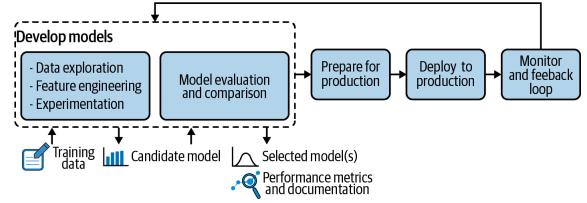
\includegraphics[width=0.66\linewidth]{images/Fig4_1_model_development.png}
\caption{Model development highlighted in the larger context of the ML project life cycle}
\end{figure}
\vspace{-0.3cm}
\begin{enumerate}\small
\item<1-> \textbf{Develop models:} Data exploration, feature engineering, experimentation, followed by model evaluation and comparison.
\item<2-> \textbf{Inputs/outputs:} Training data goes in; candidate models are produced; selected model(s) come out with performance metrics and documentation.
\item<3-> Selected models flow to \textbf{prepare for production} $\rightarrow$ \textbf{deploy to production} $\rightarrow$ \textbf{monitor and feedback loop}, which loops back to development.
\end{enumerate}
\end{frame}

%---------------------------------------------------------
\begin{frame}{Implications of Development Choices}
\begin{enumerate}
\item<1-> The implications of the \textbf{data collection process} are straightforward: a model can easily become \textbf{stale}.
\item<2-> For other parts of the model, the effects may be \textbf{less obvious}.
\item<3-> \textbf{Feature creation example:} Feeding a \textbf{date} versus a flag for \textbf{public holiday} can change performance, and also imposes different constraints on updating the model.
\item<4-> \textbf{Metrics example:} The metrics used for evaluating and comparing models may enable \textbf{automatic switching} to the best version later.
\end{enumerate}
\end{frame}

%=========================================================
\subsection{What Is a Machine Learning Model?}
%=========================================================

\begin{frame}{What Is a Machine Learning Model? --- In Theory}
\begin{enumerate}
\item<1-> An ML model is a \textbf{projection of reality}: a partial and approximate representation of some aspects of a real thing or process.
\item<2-> Once trained, it boils down to a \textbf{mathematical formula} that yields a result (a probability or a raw value) when fed inputs.
\item<3-> Models are based on \textbf{statistical theory}; ML algorithms are the \textbf{tools that build models} from training data.
\item<4-> Training data represents the world \textbf{as it was at collection time}.
\item<5-> Hence models can predict well \textbf{when the future looks like the past}.
\end{enumerate}
\end{frame}

%---------------------------------------------------------
\begin{frame}{Generalization Capacity and Examples}
\begin{enumerate}
\item<1-> \textbf{Generalization capacity:} The ability to predict accurately for cases not exactly like the input data.
\item<2-> Even outputs like \textbf{horses with zebra stripes} (CycleGAN) come from modeling a probability distribution.
\item<3-> \textbf{House price example:}
    \begin{itemize}
    \item Inputs: surface area, bedrooms, bathrooms, year of construction, location.
    \item Contextual inputs: housing market state, seller urgency.
    \item With enough historical data and stable market conditions, a reasonable estimate is possible.
    \end{itemize}
\item<4-> \textbf{Health example:} Classification models predict the \textbf{probability} of developing a disease, sometimes with a \textbf{confidence interval}.
\end{enumerate}
\end{frame}

%---------------------------------------------------------
\begin{frame}{What Is a Machine Learning Model? --- In Practice}
\begin{enumerate}
\item<1-> A model is the \textbf{set of parameters} necessary to rebuild and apply the formula.
\item<2-> It is usually \textbf{stateless and deterministic}: the same inputs give the same outputs (exception: online learning).
\item<3-> It includes \textbf{all transformations} from input data to the final formula, plus derived data (classification or decision).
\item<4-> In practice, whether ML-based or not, a model is \textbf{a computable mathematical function} applied to input data, one row at a time.
\item<5-> \textbf{House price example:} Zip codes may be replaced by derived inputs (average income, population density, amenities); this transformation is \textbf{part of the model}.
\end{enumerate}
\end{frame}

%---------------------------------------------------------
\begin{frame}{Richer Model Outputs and Packaging}
\begin{enumerate}
\item<1-> Outputs can be \textbf{richer than a single number}.
\item<2-> \textbf{Fraud detection:} Outputs a probability (maybe with a confidence interval); a \textbf{fine-tuned threshold} decides fraud classification based on costs.
\item<3-> Some models include \textbf{recommendations or decisions}: which product to show, which treatment gives the most probable recovery.
\item<4-> All transformations and associated data are part of the model, but are \textbf{not always bundled} as a single artifact.
\item<5-> Different parts have \textbf{varying constraints} (different refresh rates, external sources, etc.).
\end{enumerate}
\end{frame}

%=========================================================
\subsection{Required Components}
%=========================================================

\begin{frame}{Required Components of an ML Model (Table 4-1)}
\begin{table}
\centering
\renewcommand{\arraystretch}{1.2}
\scriptsize
\begin{tabular}{|p{2.6cm}|p{11cm}|}
\hline
\textbf{ML Component} & \textbf{Description} \\ \hline
Training data & Usually labeled with examples of what is modeled (supervised learning). Must be good data --- e.g., WWII damaged-plane data suffered from \textbf{survivor bias}. \\ \hline
Performance metric & What the model seeks to optimize; chosen carefully to avoid the \textbf{cobra effect}. If 95\% of data is class A, raw accuracy rewards always predicting A. \\ \hline
ML algorithm & Models work in various ways with pros and cons; selection depends on priorities: performance, stability, interpretability, computation cost. \\ \hline
Hyperparameters & Configurations for ML algorithms: the ways the algorithm goes to find its parameters. E.g., \textbf{depth} of a decision tree. \\ \hline
Evaluation dataset & Data different from the training set, used to evaluate performance on unseen data (\textbf{generalization}). \\ \hline
\end{tabular}
\end{table}
\begin{enumerate}\small
\item<1-> The number and complexity of these components makes good MLOps \textbf{challenging}.
\item<2-> \textbf{Algorithm choice} is yet another piece of the puzzle.
\end{enumerate}
\end{frame}

%---------------------------------------------------------
\begin{frame}{Required Components --- Explained}
\begin{enumerate}
\item<1-> \textbf{Training data:} Quality and representativeness decide model quality; biased samples (survivor bias) lead to wrong conclusions.
\item<2-> \textbf{Performance metric:} Defines ``good''; a poorly chosen metric produces unintended behavior (cobra effect).
\item<3-> \textbf{ML algorithm:} Contains the basic formula; must suit the task and priorities.
\item<4-> \textbf{Parameters vs hyperparameters:} Parameters are \textbf{learned} operations/operands of the formula; hyperparameters \textbf{guide how} they are found.
\item<5-> \textbf{Evaluation dataset:} Separate from training data to measure generalization.
\end{enumerate}
\end{frame}

%=========================================================
\subsection{Different ML Algorithms, Different MLOps Challenges}
%=========================================================

\begin{frame}{MLOps Considerations by Algorithm Type (Table 4-2)}
\begin{table}
\centering
\renewcommand{\arraystretch}{1.2}
\scriptsize
\begin{tabular}{|p{2cm}|p{2.4cm}|p{9.4cm}|}
\hline
\textbf{Algorithm Type} & \textbf{Name} & \textbf{MLOps Considerations} \\ \hline
\multirow{2}{*}{Linear} & Linear regression & Tendency for overfitting. \\ \cline{2-3}
 & Logistic regression & Tendency for overfitting. \\ \hline
\multirow{3}{*}{Tree-based} & Decision tree & Can be unstable --- small data changes can greatly change the tree structure. \\ \cline{2-3}
 & Random forest & Predictions difficult to understand (Responsible AI challenge); relatively slow to output predictions. \\ \cline{2-3}
 & Gradient boosting & Predictions difficult to understand; small changes in features or training set can radically change the model. \\ \hline
Deep learning & Neural networks & Almost impossible to interpret; extremely slow to train; need a lot of power and data. Would a simpler model work just as well? \\ \hline
\end{tabular}
\end{table}
\begin{enumerate}\small
\item<1-> All algorithms model patterns in past data; they differ in characteristics and \textbf{MLOps challenges}.
\item<2-> Quality and relevance of past experience are the \textbf{key factors} in effectiveness.
\end{enumerate}
\end{frame}

%---------------------------------------------------------
\begin{frame}{Algorithm Choice: Governance and Computing Power}
\begin{enumerate}
\item<1-> \textbf{Governance} may drive algorithm choice: regulated environments needing explanations (financial services) avoid opaque models like neural networks and favor \textbf{decision trees}.
\item<2-> Often the trade-off is on \textbf{cost}, not performance: simpler techniques need more costly \textbf{manual feature engineering}.
\item<3-> \textbf{Computing power:} ML development is \textbf{inversely proportional} to the cost of computing power.
\item<4-> New algorithms arose as compute became available; random forest and gradient boosting were expensive 20 years ago.
\item<5-> They brought \textbf{ease of use}, lowering development cost and enabling new use cases.
\item<6-> Most algorithms still operate with \textbf{all training data in memory}, not distributed big data.
\end{enumerate}
\end{frame}

%=========================================================
\subsection{Data Exploration}
%=========================================================

\begin{frame}{Data Exploration}
\begin{enumerate}
\item<1-> Data scientists must first grasp \textbf{what the data looks like}; a model is only as good as its training data.
\item<2-> Issues: \textbf{incompleteness, inaccuracy, inconsistency}.
\item<3-> Exploration processes include:
    \begin{itemize}
    \item Documenting how data was collected and assumptions made.
    \item Summary statistics: column domains, missing values, mistakes, outliers.
    \item Examining data distributions.
    \item Cleaning, filling, reshaping, filtering, clipping, sampling.
    \item Checking correlations, statistical tests on subpopulations, fitting distributions.
    \item Comparing with other data or literature.
    \end{itemize}
\item<4-> \textbf{Domain knowledge} is essential, e.g., industrial sensor data needs equipment expertise to spot abnormal outliers.
\end{enumerate}
\end{frame}

%=========================================================
\subsection{Feature Engineering and Selection}
%=========================================================

\begin{frame}{Feature Engineering and Selection}
\begin{enumerate}
\item<1-> \textbf{Features} are how data is presented to a model, informing it on things it may not infer by itself.
\end{enumerate}
\begin{table}
\centering
\renewcommand{\arraystretch}{1.2}
\scriptsize
\begin{tabular}{|p{2.5cm}|p{10.5cm}|}
\hline
\textbf{Category} & \textbf{Description} \\ \hline
Derivatives & Infer new information from existing information --- e.g., what day of the week is this date? \\ \hline
Enrichment & Add new external information --- e.g., is this day a public holiday? \\ \hline
Encoding & Present the same information differently --- e.g., day of week or weekday versus weekend. \\ \hline
Combination & Link features together --- e.g., backlog size weighted by the complexity of its items. \\ \hline
\end{tabular}
\end{table}
\begin{enumerate}\setcounter{enumi}{1}
\item<2-> \textbf{Process duration example:} From a date, derive day of week or distance to the next public holiday; consider location-specific business calendars.
\item<3-> \textbf{House price example:} Use average income and population density instead of zip code to generalize better.
\end{enumerate}
\end{frame}

%---------------------------------------------------------
\begin{frame}{Feature Engineering Techniques}
\begin{enumerate}
\item<1-> A market exists for \textbf{complementary data} beyond open data; enrichment services save time and effort.
\item<2-> \textbf{Impact coding:} Replace a modality by the \textbf{average target value} for that modality (at some information loss).
\item<3-> Most algorithms require a \textbf{table of numbers}: each row a sample, all from the same dataset.
\item<4-> \textbf{One-hot encoding:} A feature with values Raspberry, Blueberry, Strawberry becomes three yes/no features.
\item<5-> \textbf{Embeddings:} Deep learning transforms text and images into tables of numbers, enabling \textbf{transfer learning}.
\end{enumerate}
\end{frame}

%---------------------------------------------------------
\begin{frame}{Transfer Learning}
\begin{block}{Transfer Learning}
The technique of using information gained from solving one problem in solving a different problem.
\end{block}
\vspace{0.2cm}
\begin{enumerate}
\item<1-> Significantly \textbf{accelerates learning} of second or subsequent tasks.
\item<2-> Very popular in \textbf{deep learning}, where training resources can be enormous.
\item<3-> \textbf{Example:} A model trained on images without forks may still give a useful embedding for a fork detector, since it learned to detect similar \textbf{human-made objects}.
\end{enumerate}
\end{frame}

%---------------------------------------------------------
\begin{frame}{How Feature Selection Impacts MLOps Strategy}
\begin{enumerate}
\item<1-> More features may give more accuracy, more fairness, or compensate for missing information.
\item<2-> \textbf{Downsides} affecting MLOps:
    \begin{itemize}
    \item The model becomes more \textbf{expensive to compute}.
    \item More features need more inputs and \textbf{more maintenance}.
    \item Some loss of \textbf{stability}.
    \item The number of features can raise \textbf{privacy concerns}.
    \end{itemize}
\item<3-> \textbf{Automated feature selection} uses heuristics: correlation with the target, or training a simple model on a subset to find the strongest predictors.
\item<4-> Tools like \textbf{Auto-sklearn} or AutoML cross-reference features against the target to keep the most useful ones.
\end{enumerate}
\end{frame}

%---------------------------------------------------------
\begin{frame}{Human Choices and Feature Stores}
\begin{enumerate}
\item<1-> Some choices need \textbf{human intervention}, e.g., collecting additional information.
\item<2-> \textbf{Business-friendly features} improve performance, ease adoption, simplify explanations, and reduce \textbf{modeling debt}.
\item<3-> Trade-offs exist between time spent understanding the model, expected value, and risk.
\item<4-> \textbf{Feature stores:} Central repositories of features for business entities, created once and \textbf{reused}.
\item<5-> They combine an \textbf{offline} part (slower, more powerful) and an \textbf{online} part (fast, real-time), kept consistent.
\item<6-> ML is often the ``\textbf{high-interest credit card of technical debt}''; feature stores are one way to reverse this.
\end{enumerate}
\end{frame}

%=========================================================
\subsection{Experimentation}
%=========================================================

\begin{frame}{Experimentation}
\begin{enumerate}
\item<1-> Experimentation occurs \textbf{throughout} model development; important decisions are justified by experiments or research.
\item<2-> It can take many shapes: full predictive models, statistical tests, charting data.
\item<3-> \textbf{Goals of experimentation:}
    \begin{itemize}
    \item Assess how useful a model can be built given the Table 4-1 components.
    \item Find the best modeling parameters (algorithms, hyperparameters, preprocessing).
    \item Tune the \textbf{bias/variance trade-off} for a given training cost.
    \item Balance model improvement against computation cost --- how good is \textbf{good enough}?
    \end{itemize}
\end{enumerate}
\end{frame}

%---------------------------------------------------------
\begin{frame}{Bias and Variance}
\begin{enumerate}
\item<1-> \textbf{High bias (underfitting):} Fails to discover rules that could be learned from training data, due to reductive assumptions making it \textbf{overly simplistic}.
\item<2-> \textbf{High variance (overfitting):} Sees patterns in noise and predicts every variation, becoming complex and \textbf{not generalizing} beyond training data.
\item<3-> Experimentation aims to find the right balance between the two for the problem at hand.
\end{enumerate}
\end{frame}

%---------------------------------------------------------
\begin{frame}{Experimentation Tools and Budget}
\begin{enumerate}
\item<1-> Tools test possibilities \textbf{semiautomatically}: define the search space from prior knowledge and constraints (computation, budget).
\item<2-> \textbf{Stratified modeling:} Train one model per store (e.g., demand forecasting) instead of one model for all stores.
\item<3-> Trying all combinations becomes \textbf{intractable}; define a \textbf{time/computation budget} and an acceptability threshold.
\item<4-> The process may need repeating whenever data or problem constraints \textbf{change significantly}.
\item<5-> All experiments, assumptions, and conclusions may need to be \textbf{rerun and reexamined}.
\item<6-> Platforms automate workflows, preserve processing for repeatability, and support \textbf{version control and experimental branching}.
\end{enumerate}
\end{frame}

%=========================================================
\subsection{Evaluating and Comparing Models}
%=========================================================

\begin{frame}{Evaluating and Comparing Models}
\begin{enumerate}
\item<1-> George E. P. Box: \textbf{all models are wrong, but some are useful}.
\item<2-> A model should be ``\textbf{good enough to be useful}'' while avoiding the \textbf{uncanny valley} (good overall, catastrophic for a subset such as an underrepresented population).
\item<3-> Evaluate in context and \textbf{compare with what existed before} (previous model or rules-based process).
\item<4-> A disappointing absolute performance can still help, e.g., a slightly better demand forecast may give \textbf{huge cost savings}.
\item<5-> A \textbf{perfect score is suspicious}: it may indicate \textbf{data leakage} or \textbf{overfitting}.
\end{enumerate}
\end{frame}

%---------------------------------------------------------
\begin{frame}{Choosing Evaluation Metrics}
\begin{enumerate}
\item<1-> The metric chosen can lead to \textbf{very different models} (cobra effect).
\item<2-> \textbf{Accuracy} is rarely the best fit for \textbf{unbalanced classes}.
\item<3-> \textbf{Example:} If the positive class occurs 5\% of the time, always predicting negative gives 95\% accuracy but is \textbf{utterly useless}.
\item<4-> There is \textbf{no one-size-fits-all} metric.
\item<5-> Understand the metric's limits and trade-offs (\textbf{mathematics side}) and its impact on optimization (\textbf{business side}).
\end{enumerate}
\end{frame}

%---------------------------------------------------------
\begin{frame}{Cross-Testing and Cross-Validation}
\begin{enumerate}
\item<1-> \textbf{Cross-testing:} Evaluate the metric on a \textbf{holdout dataset} not used for training.
\item<2-> Data can be held out at multiple steps (metric evaluation, hyperparameter optimization).
\item<3-> \textbf{k-fold cross-validation:} Rotate held-out parts to train and evaluate multiple times; costs training time but shows \textbf{metric stability}.
\item<4-> The holdout set can be the \textbf{most recent records}, giving more realistic estimates for future predictions.
\item<5-> Recent-data holdout also helps assess whether data \textbf{drifted} between training and holdout.
\end{enumerate}
\end{frame}

%---------------------------------------------------------
\begin{frame}{Dataset Split for Model Evaluation}
\begin{columns}[T]
\begin{column}{0.50\textwidth}
\begin{figure}
\centering
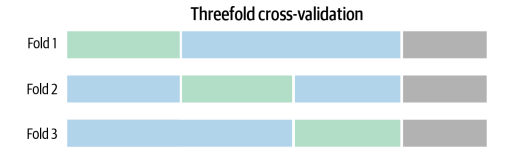
\includegraphics[width=\linewidth]{images/Fig4_2_cross_validation.png}
\caption{An example of dataset split for model evaluation}
\end{figure}
\end{column}
\begin{column}{0.48\textwidth}
\begin{enumerate}\small
\item<1-> \textbf{Gray} block: The \textbf{test (holdout) dataset}, set aside for final evaluation.
\item<2-> The remaining data is split into \textbf{three parts} (threefold cross-validation).
\item<3-> For each hyperparameter combination, the model is trained on the \textbf{blue} parts and validated on the \textbf{green} part --- three times.
\item<4-> Blue/green datasets are used with \textbf{all} combinations.
\item<5-> The gray dataset is used \textbf{only once}, with the best hyperparameter combination.
\end{enumerate}
\end{column}
\end{columns}
\end{frame}

%---------------------------------------------------------
\begin{frame}{Comparing Retrained Models}
\begin{enumerate}
\item<1-> Models are often \textbf{periodically retrained} with the same algorithms, hyperparameters, and features on more recent data.
\item<2-> Next, \textbf{compare} the new version against the previous one.
\item<3-> Also verify that \textbf{previous assumptions still hold}:
    \begin{itemize}
    \item The problem has not fundamentally shifted.
    \item Earlier modeling choices still fit the data.
    \end{itemize}
\item<4-> This is part of \textbf{performance and drift monitoring} (Chapter 7).
\end{enumerate}
\end{frame}

%---------------------------------------------------------
\begin{frame}{Cross-Checking Model Behavior}
\begin{enumerate}
\item<1-> Beyond raw metrics, understand \textbf{how the model behaves}, in proportion to its impact.
\item<2-> Ensure the model is not \textbf{actively harmful}: predicting that all patients need a doctor scores high on prevention but fails resource allocation.
\item<3-> \textbf{Reasonable steps:}
    \begin{itemize}
    \item Cross-check \textbf{different metrics}, not only the optimized one.
    \item Check reactions to different inputs (plot average prediction vs. input values).
    \item Compare behavior across \textbf{subpopulations} (e.g., error rate for males vs. females).
    \end{itemize}
\item<4-> These analyses show \textbf{correlation, not causality}; use with care for what-if analysis on unseen values.
\item<5-> Comparisons need the \textbf{full environment} (tooling, data): same settings/different data for drift, same data/different settings for performance.
\end{enumerate}
\end{frame}

%=========================================================
\subsection{Impact of Responsible AI on Modeling}
%=========================================================

\begin{frame}{Impact of Responsible AI on Modeling}
\begin{enumerate}
\item<1-> Individual predictions may need to be \textbf{explainable}: which features pushed the prediction one way or another.
\item<2-> \textbf{Shapley value:} Average marginal contribution of a feature value across all possible coalitions.
\item<3-> \textbf{Individual Conditional Expectation (ICE):} Shows the dependence between the target function and features of interest.
\item<4-> \textbf{Example:} A hormone level may indicate a health issue in general, but for a \textbf{pregnant woman} it indicates no risk.
\item<5-> Some legal frameworks mandate explainability for decisions affecting humans (e.g., \textbf{loan denial}).
\end{enumerate}
\end{frame}

%---------------------------------------------------------
\begin{frame}{Dimensions of Explainability}
\begin{enumerate}
\item<1-> Deep learning networks are called \textbf{black-box models} due to complexity.
\item<2-> Their formula is conceptually simple but \textbf{very large}, impossible to apprehend intuitively.
\item<3-> Global and local tools (partial dependence plots, Shapley values) give \textbf{insights}, but do not make the model intuitive.
\item<4-> Communicating a rigorous, intuitive understanding requires \textbf{limiting model complexity}.
\item<5-> \textbf{Fairness requirements} can also impose dimensioning constraints on model development.
\end{enumerate}
\end{frame}

%---------------------------------------------------------
\begin{frame}{Fairness Example: Weequay and Togruta}
\begin{enumerate}
\item<1-> A US-based organization trains a model to predict worker performance and hires based on it.
\item<2-> Hypothetically, everyone belongs to one of two groups: \textbf{Weequay} or \textbf{Togruta}.
\item<3-> More Weequay attend university, so Weequay applicants are \textbf{more numerous and more qualified}.
\item<4-> \textbf{Equal opportunity:} Hiring should not depend on group affiliation, all things being equal --- but this leads to more Weequay hires.
\item<5-> \textbf{Disparate impact:} Avoid practices that adversely affect one protected group more; assessed on \textbf{subpopulation proportions}.
\end{enumerate}
\end{frame}

%---------------------------------------------------------
\begin{frame}{The Fairness Trade-Off}
\begin{enumerate}
\item<1-> The two objectives are \textbf{mutually exclusive}.
\item<2-> Equal opportunity $\rightarrow$ 60\% (or more) Weequay and 40\% (or fewer) Togruta hired $\rightarrow$ \textbf{disparate impact}.
\item<3-> Forcing 40\% Togruta $\rightarrow$ some rejected Weequay were predicted more qualified $\rightarrow$ contradicts \textbf{equal opportunity}.
\item<4-> \textbf{80\% rule:} The Togruta hiring rate should be $\geq$ 80\% of the Weequay hiring rate (here, up to 65\% Weequay is acceptable).
\item<5-> Defining these objectives \textbf{cannot be a decision made by data scientists alone}.
\end{enumerate}
\end{frame}

%---------------------------------------------------------
\begin{frame}{Implementing Fairness Objectives}
\begin{enumerate}
\item<1-> Without guidance, data scientists build \textbf{equal opportunity models} (the world as it is); most tools do this.
\item<2-> \textbf{Two independent models} (one per group) may address overrepresentation, but cause \textbf{disparate treatment} --- possibly discriminatory.
\item<3-> \textbf{Post-processing:} Different thresholds per group adjust the trade-off, but may still be \textbf{disparate treatment}.
\item<4-> Bias is as much a \textbf{business question} as a technical one; there may be many protected attributes.
\item<5-> The solution depends on context: \textbf{privileges} (hiring), \textbf{negative impact} (fraud rejection), or \textbf{neutral} (disease prediction).
\end{enumerate}
\end{frame}

%=========================================================
\subsection{Version Management and Reproducibility}
%=========================================================

\begin{frame}{Version Management and Reproducibility}
\begin{enumerate}
\item<1-> Data scientists build, test, and iterate on \textbf{many model versions} and must keep them straight.
\item<2-> \textbf{Need 1 --- Experimentation:} Go back and forth on decisions, revert, and restore previous \textbf{branches} of experiments at dead ends.
\item<3-> \textbf{Need 2 --- Audit:} Data scientists, auditors, or managers may need to \textbf{replay computations} years later.
\item<4-> Versioning is largely solved for code via \textbf{source version control}; platforms offer similar features for pipelines and configurations.
\item<5-> Merging data/model branches is harder than code, but the basic need is to \textbf{return to a specific experiment} and copy its settings.
\end{enumerate}
\end{frame}

%---------------------------------------------------------
\begin{frame}{Reproducibility: Facets to Document (1/2)}
\begin{enumerate}
\item<1-> Operationalization needs model reproduction in \textbf{another environment} and possibly from a different starting point; repeatability also makes \textbf{debugging} possible.
\item<2-> \textbf{Assumptions:} Decisions about the problem, scope, and data must be explicit and logged to check against new information.
\item<3-> \textbf{Randomness:} Control pseudo-randomness via the generator \textbf{seed}; same seed gives the same sequence.
\item<4-> \textbf{Data:} The same data must be available; data versioning storage can be prohibitive, and data branching tools are less mature than code.
\item<5-> \textbf{Settings:} All processing must be reproducible with the same settings.
\end{enumerate}
\end{frame}

%---------------------------------------------------------
\begin{frame}{Reproducibility: Facets to Document (2/2)}
\begin{enumerate}
\item<1-> \textbf{Results:} Compare in-depth analyses (confusion matrices to partial dependence plots), not just text diffs.
\item<2-> \textbf{Implementation:} Slightly different implementations can yield different predictions on close calls; batch vs. live API scoring may need different implementations.
\item<3-> \textbf{Environment:} A model is more than its algorithm and parameters; a different Python package version can change results --- \textbf{freeze computation environments}.
\item<4-> Part of documentation can be \textbf{automated}; integrated design-and-deployment platforms reduce reproducibility cost.
\item<5-> Version management and reproducibility are \textbf{critical} where governance and audits matter.
\end{enumerate}
\end{frame}

%---------------------------------------------------------
\begin{frame}{Closing Thoughts}
\begin{enumerate}
\item<1-> Model development is one of the \textbf{most critical and consequential} steps of MLOps.
\item<2-> Technical decisions made here have \textbf{big repercussions} throughout the life of the model.
\item<3-> \textbf{Exposure, transparency, and collaboration} are crucial to long-term success.
\item<4-> It is the stage most practiced by data scientists.
\item<5-> In the pre-MLOps world, it often represented the \textbf{whole ML effort}, producing a model used as is, with all its consequences and limitations.
\end{enumerate}
\end{frame}
\end{document}